\chapter{Oscillators, Occupation Numbers, and the First Quantum Field}

These notes follow Leonard Susskind's sixth lecture in \emph{Advanced Quantum Mechanics}, curated by LazyingArt LLC. The lecture begins at the largest possible scale: quantum field theory is presented as the framework for essentially all known non-gravitational physics. But Susskind immediately narrows the task. Exact quantum field theories are usually too complicated to solve directly, so the evening's entry point is deliberately elementary. Before second quantization can mean anything, the harmonic oscillator has to be put back on the table, stripped of its mechanical ornament, and understood as algebra. From there the lecture unfolds in a definite sequence: one oscillator, many oscillators, occupation numbers, one-particle states in a box, and finally the operator-valued field \(\Psi(x)\) that creates and annihilates bosons at a point.

\section{Why Harmonic Oscillators Come First}

Susskind's first move is to postpone the advertised topic. Yes, the lecture is about quantum field theory and second quantization, but before either of those ideas can be useful one must review the harmonic oscillator and generalize it a little. The reason is not that springs are physically fundamental. Quite the contrary: he explicitly asks us not to think about springs very much. What matters is the algebra of the two ladder operators and the number operator built from them. That algebra is the central mathematical structure that later becomes particle creation and annihilation.

The lecture begins with the notation \(A_+\) and \(A_-\), but the same operators are more naturally written as
\[
A_+ \to a^\dagger,
\qquad
A_- \to a.
\]
We will use the dagger notation from the outset. The operator \(a^\dagger\) raises the excitation level, \(a\) lowers it, and their product is the number operator. Later these same operators will literally create and annihilate particles. At the start, however, Susskind wants the class to see only the abstract algebra and its consequences.

\section{Single-Oscillator Algebra and Energy Quanta}

For a single oscillator the lecture starts from the familiar rules
\begin{align}
a|0\rangle &= 0, \\
N &= a^\dagger a, \\
N|n\rangle &= n|n\rangle, \\
[a,a^\dagger] &= 1.
\end{align}
The state \(|0\rangle\) is the bottom state, and the states \(|n\rangle\) are eigenstates of the number operator \(N\) with eigenvalue \(n\). The operators \(a\) and \(a^\dagger\) are Hermitian conjugates of one another.

Susskind briefly reminds the audience that these operators may be written in terms of \(x\) and \(p\), but the spoken formula is self-corrected on the board and plays no real role in what follows. The lecture quickly settles on the algebraic viewpoint: once one knows \(a\), \(a^\dagger\), \(N=a^\dagger a\), and \([a,a^\dagger]=1\), one has essentially everything needed from the oscillator.

The frequency \(\omega\) survives in the Hamiltonian only as the energy cost per quantum. Up to the zero-point term,
\begin{equation}
H=\hbar\omega\left(N+\frac12\right).
\end{equation}
Throughout this lecture the additive constant \(\frac12\hbar\omega\) is set aside, so the working Hamiltonian is
\begin{equation}
H=\hbar\omega N.
\end{equation}
This is the point at which \(\omega\) really matters in the present discussion. Raising the oscillator by one level costs one unit of energy \(\hbar\omega\); lowering it returns that much energy. The harmonic oscillator is thus already a bookkeeping system for excitations counted by the integer \(n\).

\section{Many Oscillators and Occupation Numbers}

The next step is the minimal generalization that will later open the door to fields. Suppose there are many oscillators, labeled by an index \(i\), possibly infinitely many of them. Susskind's examples are deliberately simple: a collection of springs, or the infinitely many normal modes of an idealized violin string. The important point is that these are independent systems. Once that is assumed, the algebra is forced.

If two subsystems are genuinely independent, operators belonging to one must commute with operators belonging to the other. Otherwise they could not be measured independently. This gives the multimode commutation relations
\begin{equation}
[a_i,a_j]=0,
\qquad
[a_i^\dagger,a_j^\dagger]=0,
\qquad
[a_i,a_j^\dagger]=\delta_{ij}.
\end{equation}
The last relation contains the whole logic: if \(i\neq j\), the oscillators are different and the commutator vanishes; if \(i=j\), one recovers the single-oscillator commutator.

Each mode has its own number operator
\begin{equation}
N_i=a_i^\dagger a_i,
\end{equation}
and the total Hamiltonian is the sum of the energies of all modes:
\begin{equation}
H=\sum_i \hbar\omega_i N_i.
\end{equation}
Each oscillator may have its own frequency \(\omega_i\). Susskind then introduces the phrase \emph{occupation number} for the eigenvalue \(n_i\) of \(N_i\). At first it is only a name, but it is a carefully chosen name: later it will literally count how many particles occupy a given one-particle state.

A basis of states is obtained by listing the occupation number of every oscillator,
\begin{equation}
|n_1,n_2,n_3,\ldots\rangle.
\end{equation}
For a single oscillator this reduces to the usual sequence \(|0\rangle,|1\rangle,|2\rangle,\ldots\). For many oscillators it becomes a long list, finite or infinite, of nonnegative integers. The special state with no excitation anywhere is
\begin{equation}
|0\rangle = |0,0,0,\ldots\rangle,
\end{equation}
and it is annihilated by every lowering operator:
\begin{equation}
a_i|0\rangle=0
\qquad
\text{for all } i.
\end{equation}

\section{Deriving the Square-Root Factors}

At this point Susskind slows down. He does not want the ladder rules to look arbitrary, so he stops and proves the coefficient in the action of \(a^\dagger\). This pause is essential to the lecture. It turns a formal symbol into a controlled piece of mathematics.

States with different eigenvalues of \(N\) are orthogonal, and the lecture assumes the standard normalization
\begin{equation}
\langle n|m\rangle=\delta_{nm}.
\end{equation}
With that choice, \(a^\dagger|n\rangle\) cannot simply be \(|n+1\rangle\); there must be a coefficient. The board writes
\begin{equation}
a^\dagger|n\rangle=c_n|n+1\rangle.
\end{equation}
The constant \(c_n\) is to be found from the commutator.

Take the Hermitian conjugate:
\begin{equation}
\langle n|a = c_n \langle n+1|,
\end{equation}
where, as in the lecture, we choose \(c_n\) to be real. Now take the inner product of the bra equation with the ket equation:
\begin{equation}
\langle n|aa^\dagger|n\rangle
=
c_n^2 \langle n+1|n+1\rangle
=
c_n^2.
\end{equation}
The states are normalized, so the right-hand side is simply \(c_n^2\). On the left, use
\begin{equation}
aa^\dagger=a^\dagger a+1=N+1,
\end{equation}
which is the clean version of the commutator identity Susskind reaches after a brief hesitation at the board. Therefore
\begin{equation}
c_n^2=\langle n|(N+1)|n\rangle = n+1,
\end{equation}
and hence
\begin{equation}
c_n=\sqrt{n+1}.
\end{equation}
So the raising operator acts as
\begin{equation}
a^\dagger|n\rangle=\sqrt{n+1}\,|n+1\rangle.
\end{equation}

The lowering rule is obtained by the same logic, now starting from
\[
a|n\rangle=d_n|n-1\rangle.
\]
Since \(a^\dagger a=N\),
\begin{equation}
n=\langle n|N|n\rangle=\langle n|a^\dagger a|n\rangle=d_n^2,
\end{equation}
and therefore
\begin{equation}
a|n\rangle=\sqrt n\,|n-1\rangle.
\end{equation}
At \(n=0\) this automatically gives \(a|0\rangle=0\), so the formula already encodes the fact that the lowering operator annihilates the bottom state.

Susskind then lifts the result to the multimode occupation-number basis. One acts on the \(i\)-th slot exactly as for a single oscillator, leaving all other slots untouched:
\begin{align}
a_i^\dagger|n_1,\ldots,n_i,\ldots\rangle
&=
\sqrt{n_i+1}\,|n_1,\ldots,n_i+1,\ldots\rangle, \\
a_i|n_1,\ldots,n_i,\ldots\rangle
&=
\sqrt{n_i}\,|n_1,\ldots,n_i-1,\ldots\rangle.
\end{align}
This is the content of the partially visible board formula: only the \(i\)-th occupation number changes, and the familiar square root belongs to that slot alone. All other occupation numbers are merely bystanders.

A later question in the lecture asks what the square root \(\sqrt{n+1}\) ``means physically.'' Susskind's answer is revealing. Sometimes mathematics is just mathematics: the square root is what is needed for the states to remain normalized and for \(a^\dagger a\) really to act as the number operator. That is enough.

\section{From Wavefunctions to Bosonic Fock Space}

Only after the oscillator interlude is complete does Susskind return to the promised topic. But he does not define the field immediately. He first explains what the familiar wavefunction \(\psi\) is not.

For one particle, \(\psi(x)\) is the state vector in the position representation. It is not itself an observable. One does not measure the wavefunction directly; one measures position, momentum, angular momentum, and so forth. If there are several particles, then the wavefunction is not a function of one coordinate but of all particle coordinates:
\begin{equation}
\psi(x_1,\ldots,x_N).
\end{equation}
And that wavefunction describes a fixed number of particles. A fifteen-particle wavefunction describes fifteen particles, not fourteen, not sixteen. This, Susskind says, is \emph{not} the idea of a quantum field.

To build the bridge he says, in effect, ``let's go back'' to ordinary one-particle quantum mechanics. The example is a particle in a one-dimensional box. The energy eigenstates are a family of one-particle wavefunctions
\begin{equation}
\psi_1(x),\ \psi_2(x),\ \psi_3(x),\ \ldots,\ \psi_i(x),
\end{equation}
ordered by energy. The first is the smoothest function that fits in the box, the next has one node, and higher states oscillate more rapidly. If one wishes to keep a standard model in mind, the ideal infinite well would use
\begin{equation}
\psi_n(x)=\sqrt{\frac{2}{L}}\sin\!\left(\frac{n\pi x}{L}\right),
\qquad 0<x<L,
\end{equation}
but the lecture itself relies only on the qualitative ordering by increasing node count and energy.

\begin{figure}[ht]
\centering
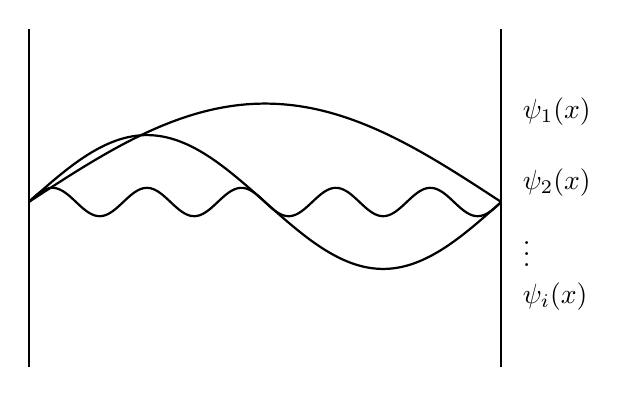
\begin{tikzpicture}[x=1cm,y=1cm]
\draw[thick] (0,0) -- (0,4.3);
\draw[thick] (6,0) -- (6,4.3);

\draw[thick,domain=0:6,samples=120] plot (\x,{2.1+1.25*sin(180*\x/6)});
\draw[thick,domain=0:6,samples=120] plot (\x,{2.1+0.85*sin(360*\x/6)});
\draw[thick,domain=0:6,samples=240] plot (\x,{2.1+0.18*sin(1800*\x/6)});

\node[right] at (6.15,3.25) {$\psi_1(x)$};
\node[right] at (6.15,2.35) {$\psi_2(x)$};
\node[right] at (6.15,1.55) {$\vdots$};
\node[right] at (6.15,0.90) {$\psi_i(x)$};
\end{tikzpicture}
\caption{Qualitative one-particle box modes, redrawn from the lecture sketch. What matters here is the ordering of modes and their increasing oscillation, not precise amplitudes.}
\end{figure}

Now the earlier oscillator language suddenly reappears. Suppose there are many bosons, of not necessarily fixed total number, occupying these one-particle states. Then a basis of many-body states is obtained by specifying how many particles occupy each one-particle mode:
\begin{equation}
|n_1,n_2,n_3,\ldots\rangle.
\end{equation}
The resemblance to the many-oscillator basis is not accidental. It is the central structural observation of the lecture. Each one-particle state behaves as though it were its own oscillator, and the occupation number of that oscillator is literally the number of bosons occupying that state.

This is also where the creation and annihilation operators acquire their particle interpretation. Acting with \(a_i^\dagger\) increases the number of particles in the \(i\)-th one-particle state by one; acting with \(a_i\) decreases it by one. The same oscillator algebra is now particle bookkeeping.

The free many-body Hamiltonian is therefore
\begin{equation}
H=\sum_i \omega_i a_i^\dagger a_i.
\end{equation}
Here \(\omega_i\) is the energy of a particle in the \(i\)-th one-particle state, after Susskind has dropped \(\hbar\) from the notation. The question period after the break settles several possible confusions about this formula.

First, the \(\omega_i\) need not be equally spaced. The energy levels of a particle in a box are not harmonic-oscillator levels. What is evenly spaced is something else: for a fixed mode \(i\), the sequence of occupation numbers \(0,1,2,\ldots\) forms the equally spaced ladder associated with that oscillator.

Second, the particles are free. That is why the total energy is additive. If the particles interacted, one would have to include interaction energy and the Hamiltonian would not be just a sum of one-particle contributions.

Third, the omitted zero-point constant really is irrelevant at this stage. Adding a constant \(C\) to the Hamiltonian changes no commutator:
\begin{equation}
[O,H+C]=[O,H].
\end{equation}
So the equations of motion are unchanged, and only energy differences matter in the present discussion.

The variable-particle-number space spanned by the states \(|n_1,n_2,\ldots\rangle\) is what the lecture identifies as Fock space. It is this space, not the fixed-\(N\) wavefunction space, on which the quantum field will act.

\section{The Nonrelativistic Field Operator and What It Does}

Only now, after all of these preparations, does Susskind give the definition. He explicitly warns the class not to demand too much intuition too early. Definitions are judged by what they let one do. In that spirit the nonrelativistic bosonic field is introduced as
\begin{equation}
\Psi(x)=\sum_i a_i\,\psi_i(x),
\end{equation}
with Hermitian conjugate
\begin{equation}
\Psi^\dagger(x)=\sum_i a_i^\dagger\,\psi_i^*(x).
\end{equation}
The \(\psi_i(x)\) are ordinary one-particle wavefunctions, just numbers once \(x\) is specified. The operator character lives entirely in the \(a_i\) and \(a_i^\dagger\). Thus for each spatial point \(x\) there is an operator \(\Psi(x)\) acting on Fock space.

This is also where the earlier question about Fourier analysis finds its answer. If the one-particle basis is taken to be momentum eigenstates, then the \(\psi_i(x)\) are plane waves or trigonometric modes, and the operators \(a_i\) play the role of quantum Fourier coefficients. More generally, the field is expanded in whatever complete orthonormal basis of one-particle states is convenient.

Susskind first motivates \(\Psi\) as the kind of quantity one would like to regard as observable. A few minutes later he corrects the point himself: \(\Psi\) and \(\Psi^\dagger\) are not Hermitian, so taken separately they are not observables in the strict quantum-mechanical sense. The mathematically careful statement is that \(\Psi\) is an operator-valued field, and Hermitian combinations such as \(\Psi+\Psi^\dagger\), or densities built from them, are the observable quantities. The main point of the lecture, however, is not this distinction but what the field does.

\subsection{Action on the vacuum}

The first calculation is the one Susskind wants the audience to remember. What does \(\Psi^\dagger(x)\) do to the vacuum?

Let \(|i\rangle\) denote the one-particle state with wavefunction \(\psi_i(x)\), so that
\begin{equation}
\langle x|i\rangle=\psi_i(x).
\end{equation}
Because the \(|i\rangle\) form a complete basis of one-particle states,
\begin{equation}
\sum_i |i\rangle\langle i|=1.
\end{equation}
Apply this identity operator to the position eigenstate \(|x\rangle\):
\begin{align}
|x\rangle
&=
\sum_i |i\rangle\langle i|x\rangle \\
&=
\sum_i \psi_i^*(x)\,|i\rangle.
\end{align}
Now rewrite the one-particle state \(|i\rangle\) in Fock-space language. It is created from the vacuum by
\begin{equation}
|i\rangle=a_i^\dagger|0\rangle.
\end{equation}
Substituting,
\begin{align}
|x\rangle
&=
\sum_i \psi_i^*(x)\,a_i^\dagger|0\rangle \\
&=
\Psi^\dagger(x)|0\rangle.
\end{align}
This is the payoff of the definition:
\begin{equation}
\Psi^\dagger(x)|0\rangle=|x\rangle.
\end{equation}
The field operator \(\Psi^\dagger(x)\) creates a particle at position \(x\).

By contrast,
\begin{equation}
\Psi(x)|0\rangle=0,
\end{equation}
because every term in \(\Psi(x)\) contains an annihilation operator. The field \(\Psi(x)\) removes a particle at \(x\), and if there is none to remove, the result is the zero vector.

\subsection{Vacuum versus zero}

Susskind dwells on this point because the notation is treacherous. The vacuum \(|0\rangle\) is not the zero vector. It is a normalized state, of norm one, representing empty space in this simplified theory. The symbol \(0\) in \(|0\rangle\) means zero particles, not zero length.

When an annihilation operator acts on the vacuum, the result is the genuine zero vector,
\begin{equation}
a_i|0\rangle=0.
\end{equation}
That vector has zero norm and cannot be normalized. It does not describe a physical state. The lecture spends time emphasizing this because the distinction matters. A superposition of the vacuum with a one-particle state is a meaningful state with indefinite particle number. Adding the zero vector to a state changes nothing at all.

\subsection{Two particles and bosonic symmetry}

Once \(\Psi^\dagger(x)\) is understood as ``put a particle at \(x\),''
the two-particle state is obtained by acting again:
\begin{equation}
\Psi^\dagger(y)\Psi^\dagger(x)|0\rangle.
\end{equation}
Expanding both fields gives
\begin{equation}
\Psi^\dagger(y)\Psi^\dagger(x)
=
\sum_{i,j} a_i^\dagger a_j^\dagger\,\psi_i^*(y)\psi_j^*(x).
\end{equation}
But all creation operators commute,
\begin{equation}
[a_i^\dagger,a_j^\dagger]=0,
\end{equation}
so the field operators commute as well:
\begin{equation}
[\Psi^\dagger(x),\Psi^\dagger(y)]=0.
\end{equation}
Therefore
\begin{equation}
\Psi^\dagger(y)\Psi^\dagger(x)|0\rangle
=
\Psi^\dagger(x)\Psi^\dagger(y)|0\rangle.
\end{equation}
This is exactly the symmetry of bosons under exchange. In the lecture Susskind points out that one could almost reverse the logic: had one started with this construction alone, the symmetry would have shown that the particles produced in this way are bosons.

A single field \(\Psi\) describes a single species of boson. Different bosonic species require different fields. The spatial argument tells the field where to create or annihilate the particle; the field itself tells us what kind of particle it is.

\subsection{Why this formalism is useful}

The lecture closes by returning to motivation. If one were studying a world with exactly thirty-seven particles, never thirty-six and never thirty-eight, then this machinery would be an unnecessarily elaborate detour. But quantum field theory is designed for a different problem: systems in which the particle number may vary, and even states that are superpositions of different particle numbers. In that sense it is, as Susskind says, a bookkeeping device, though an extremely powerful one.

In particular, the formalism naturally describes states built from
\[
|0\rangle,\qquad
\Psi^\dagger(x)|0\rangle,\qquad
\Psi^\dagger(y)\Psi^\dagger(x)|0\rangle,
\qquad \text{and so on,}
\]
and also superpositions of sectors with different numbers of particles. A laser field is the lecture's example: not a state of a definite number of photons, but a superposition of many photon-number sectors. That is precisely the sort of situation for which the field-operator language is meant.

\section{Summary}

The lecture enters quantum field theory by a deliberate sequence of reductions and reinterpretations. First, the harmonic oscillator is recast as pure operator algebra. Then many independent oscillators are organized by occupation numbers. Next, a one-particle basis in a box is reinterpreted as a family of modes that can each be occupied by any number of bosons. Only after that preparation does the field appear:
\begin{equation}
\Psi(x)=\sum_i a_i\psi_i(x),
\qquad
\Psi^\dagger(x)=\sum_i a_i^\dagger\psi_i^*(x).
\end{equation}

The relation between particles and fields is then no longer mysterious. The operator \(\Psi^\dagger(x)\) acting on the vacuum creates a particle at \(x\), repeated action creates multiparticle states, and the commutativity of the creation operators makes those particles bosons. What began as oscillator algebra has become a formalism for states with indefinite particle number. That is the lecture's central lesson: in this simplest nonrelativistic setting, quantum field theory is the natural language for counting, creating, annihilating, and superposing quanta.